% #############################################################################
% This is Chapter 4
% !TEX root = ../main.tex
% #############################################################################
% Change the Name of the Chapter i the following line
\fancychapter{Architecture}
\cleardoublepage
% The following line allows to ref this chapter
\label{chap:arch}

The fundamental objective of the system was to develop a portable device which enables users and entities to establish safe channels of communication.
A solution was developed on a portable \ac{HSM}, which secures communications between users, saves the owners's sensitive data, such as keys and documents, and performs all security critical operations. This is an easy process for the owner, who does not need to worry about any setup or management, the system is acessible and ready to use, when delivered.
This chapter presents an overview of the developed system, the relevant services and end user use cases.

% The system is designed so that each user, either an individual or entity, has it's own physical device.

% -----------------------------------------------------
% -----------------------------------------------------
\section{Overview}\label{chap:arch:overview}

The system, pictured in figure~\ref{fig:overview}, is composed of two main components: the physical device, responsible for all operations, and the client software on the user's computer, which provides a simple interface to the user.

\begin{figure}[h]
    \centering
    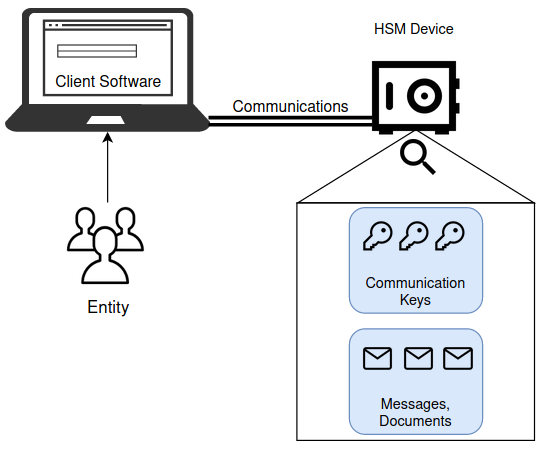
\includegraphics[width=0.75\textwidth]{./Images/overview.png}
    \caption{System Overview}
    \label{fig:overview}
\end{figure}

The client's computer running the software, is connected to the device through a physical connection, used to send and receive data and commands. A simple application for the client's computer was developed to interface with the device.
Using these tools, the entity can signal the device to perform the desired operations.
The implemented services are available inside the device, which stores and manages keys, as well as documents.
If the device is misplaced or stolen, the stored keys and documents are not at risk of being compromised or extracted. The developed software and physical tamper measures ensure it.
% All data is either stored in the secure eNVM portion, or in the non-volatile memory, encrypted with an internal \ac{KEK}.

Upon receiving their device, each user is only required to plugin it into a power socket, and to their computer using the appropriate cable, and the system is ready to use, through the provided client software.

% -----------------------------------------------------
% -----------------------------------------------------
\section{Services}\label{chap:arch:services}

This section will define and describe the system services for the end user.
Firstly it presents the authentication, then main services, divided in their objective, secure data exchange or new communications.

Any user needs to be authenticated through a \ac{PIN} number in order to access the system operations. This way, each entity with multiple users can organically handle which users are authorized to handle the system by handing out the corresponding \ac{PIN} number.
The device comes from fabric with a default authentication \ac{PIN}, which is supplied to the owners. It can be changed at any time by an authenticated user.
To authenticate himself to the device, the user sends a \ac{PIN} through the software, the device then compares it to the authentication number securely stored inside it. Once authenticated, the session will be unlocked, and the user will be able to perform operations.

% -----------------------------------------------------
\subsection{Initial State}\label{chap:arch:services:initial-state}

The device will come from fabric configured and prepared with the necessary keys to secure communications.
Before acquiring the device, each entity can provide a list of entities whom they wish to securely communicate. The device will then be delivered to each entity with the necessary keys. This allows owners to begin to communicate immediately, with no setup necessary.
Additionally the device is delivered with the necessary functionality and keys, so all devices can establish new communications with new entities. This provides the flexibility of secure data exchange with a new entity, without having to send the device back to the control station or fabric, to be loaded with the necessary keys.
% depending on two scenarios. In the simpler scenario, the device comes with the symmetric keys already shared and stored in each entities' device.
% In the other scenario, the entities will receive the device with a pair of asymmetric keys, a private and public, generated inside the device from fabric. Each device will have the user's public keys, whom he wishes to communicate. The entity can request whose public keys he wants, before the device is initialized in fabric. This allows the users to share symmetric keys between them, which they can user to begin trading data securely.

% -----------------------------------------------------
\subsection{Secure Data Exchange}\label{chap:arch:services:data}

The main operations are responsible fore securing the communications between users. These operations will grant confidentiality, integrity and authentication to communications.
% The main operations are responsible fore securing the communications between users. These operations will grant confidentiality, integrity, authentication and non-repudiation to communications.

% \begin{figure}[h]
%     \centering
%     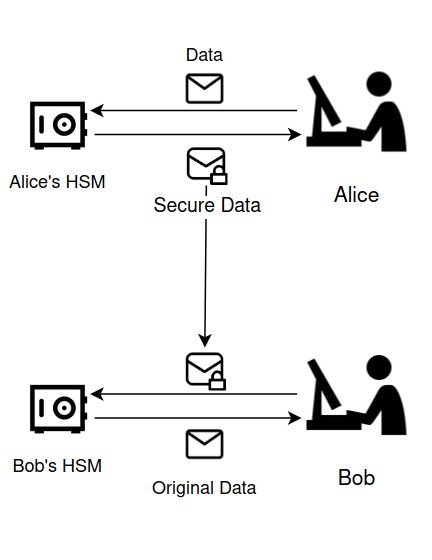
\includegraphics[width=0.5\textwidth]{./Images/arch-data-service.png}
%     \caption{Secure data exchange service using internal keys usage example}
%     \label{fig:arch:data-service}
% \end{figure}

% The secure data exchange services are divided in two. The first provides \textbf{confidentiality} and \textbf{authentication} to a piece of data, such as a document.
The secure data exchange services provides \textbf{confidentiality} and \textbf{authentication} to a piece of data, such as a document.
An usage example of secure data exchange is depicted in figure \ref{fig:arch:data-service}. Firstly, Alice forwards the data, to be sent securely to Bob, to the device through the software and the device returns the data secured with an internal key. Then, Alice can forward the result to any entity with the same internal key, through a chat application, e-mail or other convenient service.
The receiver Bob sends the secure data to the device, and receives the original message.
This service prevents any third party from gaining access to the data, or altering the message. The receiver can be confident of the data's origin. It could not have been sent by any malicious entity.

% Qualified digital signatures provide \textbf{non-repudiation} to a piece of data, using the private key generated inside the box. The user sends the data to the box, and the subsequent signature will be returned as pictured in figures~\ref{fig:arch-ds} and~\ref{fig:arch-ds-verify}.

% -----------------------------------------------------
\subsection{New Communications}\label{chap:arch:ops:new}

As introduced before, the device provides the flexibility to establish communications with other entities, even new ones, not previously requested by the user.
The device can also import a new set of keys, provided by the control station.
This way already established channels of communication can be updated in a regular time schedule defined by the entities, in other to maintain secure communications, with the desired entities.

When a user wants to communicate with a new entity, the system provides two convenient solutions. The user can securely contact the control station at any time to request the public information of the other entity, through the secure data exchange service, equivalent to communicating with any other entity.
Then the user needs to send the information through the client software to the device. The new key is generated in the device and made available right away. Then data can be exchanged with the new entity, which must also request the control station for the analogous entity's public information.
This service allows establishing connections with new entities when needed, by way of trusted third party, the control station. 

% \begin{figure}[h]
%     \centering
%     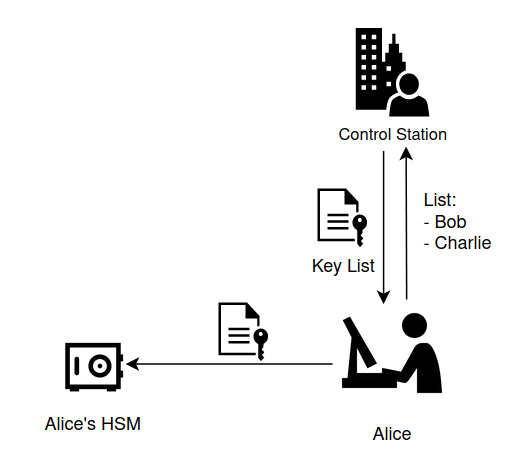
\includegraphics[width=0.65\textwidth]{./Images/arch-import-service.png}
%     \caption{Import key list to device usage example}
%     \label{fig:arch:import-service}
% \end{figure}

The system can also be setup with a regular communication update schedule. It grants the flexibility of key revocation when needed, data exchange with new entities, as well as updating communication keys which have reached their expiration date, with no additional complexity to the user, to always safeguard the security of communications.
Each month an entity can hand over a list of the entities it wishes to communicate with to the control station, which will accordingly yield the corresponding key set, as pictured in figure \ref{fig:arch:import-service}.
Each entity only needs to forwards the list to the device, and the new keys are immediately stored and ready to be used.
Users can resume communications, same way as before with minimal interruption, with the requested entities.

% When a symmetric key is revocated, due to reaching its expiration date, or from being compromised, entities can generate a new one, using the aforementioned procedure, with an additional parameter for the key derivation function, to generate a completely new and unique key.
% Import
% Generate

% Supported management operations include generation of new symmetric keys for communication and revocation of existing keys saved in the device, if communications are suspected to be compromised.
% These operations are only available in the scenario where each device has a pair of asymmetric keys, and there is a protocol in place to distribute public keys.

% An entity receives their device, prepared to communicate with other entities, and a list of information of other entities, available to create communications. This information, namely the entities public key, can be imported into the device to generate new keys.
% After the key is imported, a secure connection with a new entity can be established, by sharing symmetric keys.
% In order for an entity to communicate with a another entity, with no previously established communications, their device will generate a new symmetric key and store it in secure storage, or in non-volatile memory, encrypted with the device's public key.

% -----------------------------------------------------
\section{Summary}\label{chap:arch:summary}

This section described the system's functionalities in a practical approach with examples for end users.
The system grants secure communications between any number of users, as soon as they receive the device, without overloading the users with convoluted tasks or responsibilities.
It is very flexible in allowing entities to manage the authorized user's to their devices and with whom they wish to communicate, by offloading this management component and responsibility to a trusted control station.
